%%%%%%%%%%%%%%%%%%%%%%%%%%%%%%%%%%%%%%%%%%%%%%%%%%
\begin{frame}{Overview}

\Large{Specification by Example}

\vspace{2em}

\begin{itemize}
	\item Motivation

	\item Goal

	\item Path

	\item Example
\end{itemize}

\end{frame}


%%%%%%%%%%%%%%%%%%%%%%%%%%%%%%%%%%%%%%%%%%%%%%%%%%
\begin{frame}{Software From Different Perspectives}

\begin{itemize}

	
	\item Customer:

	\begin{itemize}
		\item \glqq The software should do what I expect.\grqq
		\item \glqq I want the software to be good value for money.\grqq
	\end{itemize}
	
	
	\item Developer:
	
	\begin{itemize}
		\item \glqq I want to know what I sould develop.\grqq
		\item \glqq When am I done?\grqq
	\end{itemize}
	
	
	\item After delivery:
	
	\begin{itemize}
		\item \glqq What exactly does the software do?\grqq
		\item \glqq Bug or feature?\grqq
	\end{itemize}
\end{itemize}

\end{frame}


%%%%%%%%%%%%%%%%%%%%%%%%%%%%%%%%%%%%%%%%%%%%%%%%%%
\begin{frame}{The Vision -- One Source for Everybody}

\begin{itemize}
	\item Description of a requirement

	\item Acceptance tests for development

	\item Executable documentation
\end{itemize}

\vspace{1em}

$\Rightarrow$ Single Source of Truth

\end{frame}


%%%%%%%%%%%%%%%%%%%%%%%%%%%%%%%%%%%%%%%%%%%%%%%%%%
\begin{frame}{How do we get there}


\begin{itemize}
	\item Communication and discussion \em of all \em participants 
	
	\item Focus on the business aspects
\end{itemize}


\vspace{1em}

$\Rightarrow$ Specification Workshops

\end{frame}



%%%%%%%%%%%%%%%%%%%%%%%%%%%%%%%%%%%%%%%%%%%%%%%%%%
\begin{frame}{A Typical Specification Workshop}

\begin{itemize}
	\item The customer describes the problem he wants to solve
	\item The other participants question him to gain clarity
	\item Together all participants create examples
        \item In case of many participants: Create examples in small groups
	\item The examples are condensed and reduced to focus on the essentials
	\item The underlying specification is derived from the examples
\end{itemize}

\end{frame}



%%%%%%%%%%%%%%%%%%%%%%%%%%%%%%%%%%%%%%%%%%%%%%%%%%
\begin{frame}{Be Wary of These}

\begin{itemize}
   \item Complicated examples
   
   \item Naming
   
   \item Formulae
\end{itemize}


\end{frame}



%%%%%%%%%%%%%%%%%%%%%%%%%%%%%%%%%%%%%%%%%%%%%%%%%%
\begin{frame}{From the Examples to the Specification}

\begin{itemize}
	\item The specification is derived from the examples (summarising)
	\item Specification is checked against the introductory questions
	\item This way, completeness can be checked in both directions
	\item Must be understandable by somebody who did not participate in the workshop
\end{itemize}

\end{frame}
 
%%%%%%%%%%%%%%%%%%%%%%%%%%%%%%%%%%%%%%%%%%%%%%%%%%
\begin{frame}{Example: Concrete Requirement}

\begin{itemize}
      	\item I am the owner of a hot dog stand, and I have a small cash register system with inventory management
	\item I want the system to automatically order fresh supplies whenever I run out of sausages

\end{itemize}
	
$\Rightarrow$ Please create examples in small groups (about 4 persons)!

\end{frame}

%	\item What I already know:
%	\begin{itemize}
%		\item My supplier takes at most 30 minutes
%		\item On Tuesdays I sell more hot dogs
%		\item After 16:00 h I do not sell much any more
%	\end{itemize}
%
%	\item Currently, I order in this way:	
%	\begin{itemize}
%		\item When my supplies reach 10 sausages (on Tuesdays: 20)
%		\item Only before 16:00 h
%	\end{itemize}


%%%%%%%%%%%%%%%%%%%%%%%%%%%%%%%%%%%%%%%%%%%%%%%%%%
\begin{frame}{Beispiel 1}

\begin{center}
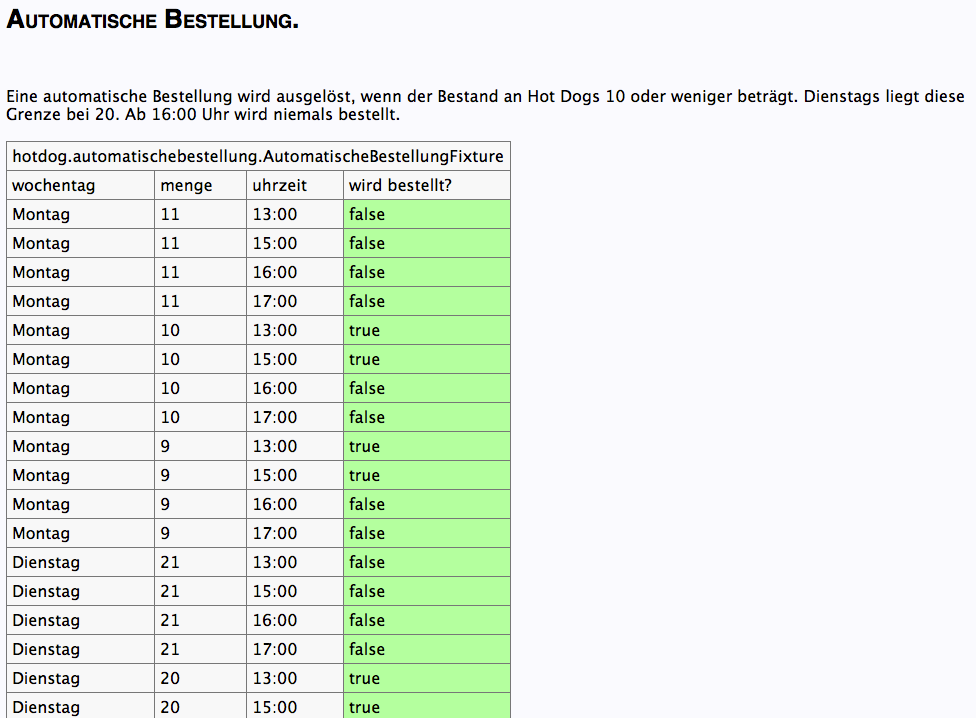
\includegraphics[height=7cm]{SchlechtesBeispiel.png} \newline
\end{center}

\end{frame}

%%%%%%%%%%%%%%%%%%%%%%%%%%%%%%%%%%%%%%%%%%%%%%%%%%
\begin{frame}{Beispiel 2}

\begin{center}
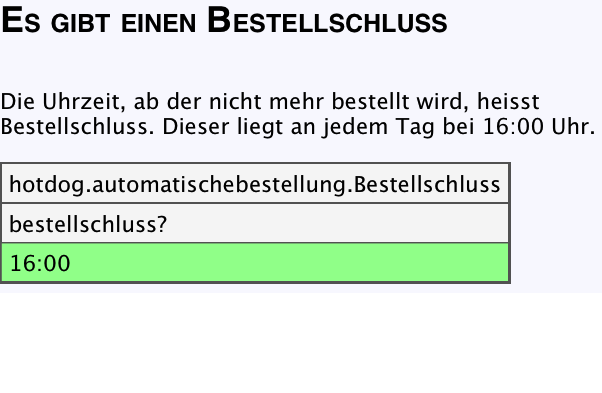
\includegraphics[width=5cm]{bestellschluss.png}
\hfill{}
\onslide+<2->
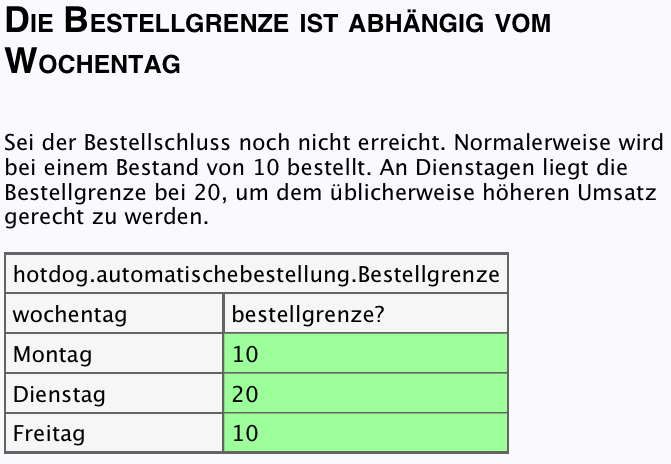
\includegraphics[width=5cm]{wochentag.png}
 \newline
\onslide+<3->
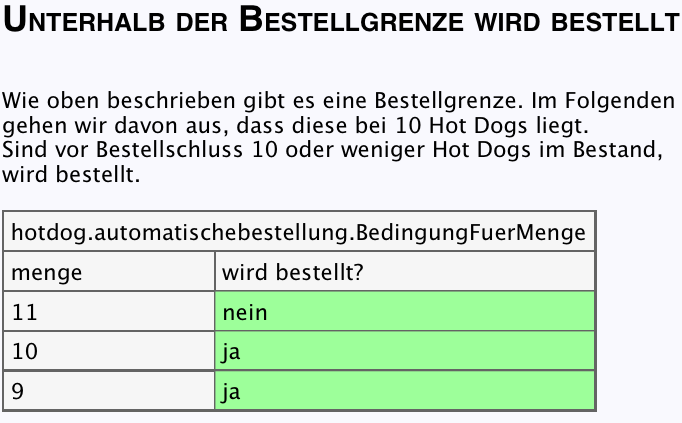
\includegraphics[width=5cm]{bestellgrenze.png}
\hfill{}
\onslide+<4->
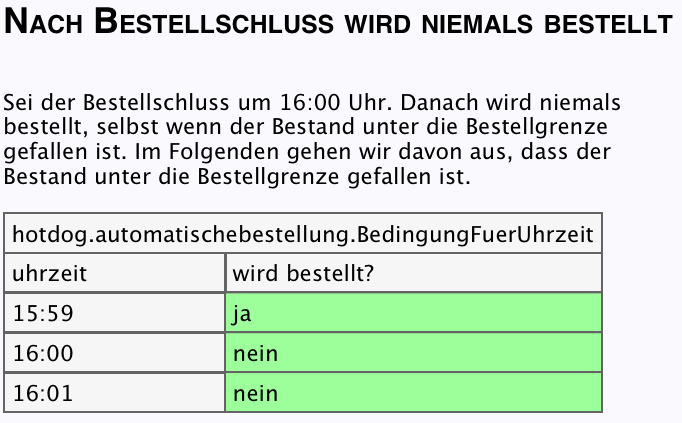
\includegraphics[width=5cm]{keineBestellungNachBestellschluss.png} 
\end{center}

\end{frame}

%%%%%%%%%%%%%%%%%%%%%%%%%%%%%%%%%%%%%%%%%%%%%%%%%%
\begin{frame}{Fazit}

\begin{itemize}
	\item Central Aspect: Communication in the Specification Workshop
	\item Central results:
	\begin{itemize}
		\item Business model of the domain
		\item Executable Examples (i.e.~tests)
	\end{itemize}
	\item Specification is important for everybody (customer, developer, QA, support)
	\item Then it is possible to have one source for requirements and documentation that is connected to the application
\end{itemize}

\end{frame}

%%%%%%%%%%%%%%%%%%%%%%%%%%%%%%%%%%%%%%%%%%%%%%%%%%
\begin{frame}{Books regarding the Subject}

\begin{center}
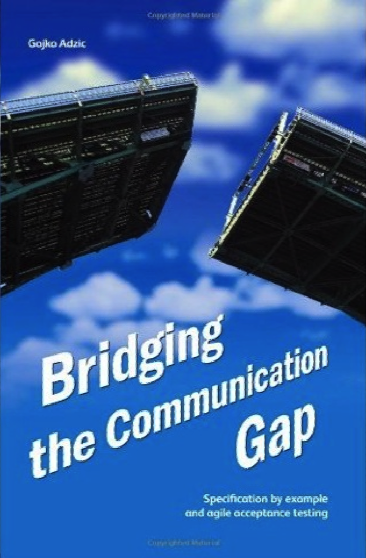
\includegraphics[height=7cm]{CommunicationGap.png}
\hfill

\includegraphics[height=7cm]{SpecificationByExample.png}
\end{center}

\end{frame}

%%%%%%%%%%%%%%%%%%%%%%%%%%%%%%%%%%%%%%%%%%%%%%%%%%
{
\usebackgroundtemplate{
\includegraphics[width=\paperwidth,height=\paperheight]{background-slide.png}}
\begin{frame}{Many Thanks!}

        Slides on GitHub:
        \vspace{-0.8em}
        \begin{center}
                \url{https://github.com/leider/Beispielhaft}
        \end{center}

        \begin{block}{Andreas Leidig}
        \begin{description}[Twitterxx]
                \item[E-Mail]  \href{mailto:andreas.leidig@msg-gillardon.de}{\texttt{andreas.leidig@msg-gillardon.de}}
                \item[Twitter] \href{http://twitter.com/leiderleider}{\texttt{@leiderleider}}
        \end{description}
        \end{block}

        \begin{block}{Nicole Rauch}
        \begin{description}[Twitterxx]
                \item[E-Mail]  \href{mailto:nicole.rauch@msg-gillardon.de}{\texttt{nicole.rauch@msg-gillardon.de}}
                \item[Twitter] \href{http://twitter.com/NicoleRauch}{\texttt{@NicoleRauch}}
        \end{description}
        \end{block}
\end{frame}
}

%%%%%%%%%%%%%%%%%%%%%%%%%%%%%%%%%%%%%%%%%%%%%%%%%%
%\begin{frame}{Quellen}
%
%\begin{itemize}
%\item Kompliziert.jpg: 
%\url{http://chestofbooks.com/crafts/metal/Elementary-Metal-Work/Nails-And-Nailed-Strips.html}
%\item Formeln.jpg: 
%\url{http://depts.washington.edu/ecnboard/wordpress/wp-content/uploads/2011/01/math_image-300x269.jpg}
%\item Namen.jpg: 
%\end{itemize}
%
%\end{frame}
